\documentclass[english,aps,pra,amsmath,amssymb,showpacs,notitlepage,onecolumn]{revtex4-1}
%\usepackage{epsfig}
\usepackage{amsmath}
\usepackage{mathtools}
\usepackage[svgnames]{xcolor}
\usepackage[colorlinks=true, linkcolor=Maroon, urlcolor=Blue]{hyperref} 
%\usepackage{sidecap}
\usepackage{microtype}
\DisableLigatures{encoding = *, family = *}
\usepackage[figuresleft]{rotating}
%\usepackage{caption}
\usepackage{float}
\usepackage{subfigure}
\usepackage{graphicx}
\hypersetup{
  colorlinks,
  citecolor=MidnightBlue,
  linkcolor=DarkRed,
  urlcolor=Blue}
% \usepackage{lscape}
\newcommand{\EssD}{\mathcal{D}}
\def\etal{{\it et al. }}
\def\prb{Phys. Rev. B }
\def\pra{Phys. Rev. A }
\def\prl{Phys. Rev. Lett. }
\def\pla{Phys. Lett. A }
\def\pb{Physica B}
\def\ajp{Am. J. Phys. }
\def\mpl{Mod. Phys. Lett. B }
\def\ijmp{Int. J. Mod. Phys. B}
\def\ijp{Ind. J. Phys. }
\def\ijpap{Ind. J. Pure Appl. Phys. }
\def\ibmjrd{IBM J. Res. Dev. }
\def\pjp{Pramana J. Phys.}

\begin{document}
\title{Playing a true Parrondo's game with a three state coin on a quantum walk}
\author{Jishnu Rajendran}
\author{Colin Benjamin}
\email{colin.nano@gmail.com}
\affiliation{School of Physical Sciences, National Institute of Science Education \& Research, HBNI, Jatni-752050,\ India }
\begin{abstract}
A coin with three states is not necessarily an anomaly. A coin falls on either of its two sides head or tail. However, there is a remote possibility that it may not fall but roll on its edge and get stuck somewhere without falling on either of its sides. This possibility is remote for a classical coin so much so that it is never analyzed. For a three-state quantum coin(qutrit), this is a fact. It has three states, period. Playing a Parrondo's game with a qutrit is the subject of this paper. We show that a true quantum Parrondo's game can be played with a 3 state coin in a 1D quantum walk in contrast to the fact that playing a true Parrondo's game with a 2 state coin(qubit) in 1D quantum walk fails in the asymptotic limits.

\end{abstract}
\maketitle
\section{Introduction}
Quantum walks(QW), motivated from classical random walks, have proven to be of great utility in simulating many physical systems \cite{two_particle,Marquez-Martin2016} as well as in developing better quantum algorithms \cite{algo,qcomp1,qcomp2}, so as universal computational primitive\cite{universal}. Similar to a classical random walk, quantum walk can be described in a one-dimensional lattice with walker starting from the origin, however, unlike the classical random walk here the walker is described quantum mechanically by a wavefunction. Similar to a classical random walk, quantum walks consist of a walker and a coin. In case of classical random walks, the walker starts from origin moves left or right according to a coin toss, say if the coin toss yields head the walker moves right otherwise moves left. Probability distribution of the classical random walk in a one-dimensional lattice after $n$ steps is a \textit{binomial distribution} \cite{classical}. In case of quantum walks the walker is a quantum object. The coin corresponding to a quantum walker in case of a two-state(head and tail) coin is a qubit. Similar to the classical random walks, in quantum walks if the coin toss yields head the walker moves towards right otherwise left. In addition to head or tail, the coin in quantum case can be in a superposition of head and tail and then walker will move to a corresponding superposition of left and right lattice sites. The probability distribution of the quantum walk is a two-peaked distribution peaking around the two edges, which is evidently different from that of classical random walk where peak is at origin\cite{Andraca}. Similar to a quantum walk with two state coin(qubit), one can devise a quantum walk with a three-state coin too which is a qutrit. Quantum walks with qutrits have been attempted before in the context of localization \cite{qutrit1}and coin eigenstates\cite{qutrit2} . Qubits are the quantum analogue for head and tail, similarly, qutrit is the quantum analogue of a three-state coin with a head, tail and side as shown in the Figure \ref{classical_coin}. Similar to the two-state coin quantum walk described above, for a three-state quantum walk, if the coin lands on its head the walker moves right, if on tails walker moves to left and if the coin falls on side then the walker stays in the same position. In case of classical random walk the walker with three state coin moves toward right when the coin lands on its head, moves left when coin lands on its tail but there is also a small probability that the coin falls on its side, then the coin toss is repeated this is one way of making analogy with the quantum walk with qutrit(three state coin).\\


The relevance of game theory spreads throughout many scientific fields. Quantum effects introduced to the classical game theory led to the development of quantum game theory, where the probabilities are taken in to account with quantum effects like superposition and interference\cite{q_game}. Parrondo's games\cite{parrondo}, in its simplest form, is a gambling game consisting two games A and B. whose outcome is determined by the toss of a biased coin. When a player plays each of them individually results in losing whereas if played alternatively can result in a winning outcome. This apparent paradox when each of these games is losing when played individually but when played alternately or in some other deterministic or random sequence (such as $ABB\ldots$,$ABAB\ldots$, etc.) can become a winning game is known as Parrondo's paradox. Originally J.~M.~R.~Parrondo devised this paradox to provide a mechanism for Brownian ratchets where a directed motion can be harnessed from Brownian motion. The previous attempt for a Parrondo's paradox with a single coin qubit on quantum walks failed in asymptotic limits\cite{minli,flitney}. In one of our previous works, we showed a genuine quantum Parrondo's paradox in the asymptotic limits not with a single coin but with two coins\cite{previous}.In this work, our aim is to replicate the quantum Parrondo's paradox in asymptotic limits in a quantum walk not with two coins but with a single three-state coin as described above in the first paragraph. The paper is organized in the following manner, starting with a brief introduction and motivation, in section \ref{2state} we discuss how Parrondo's games cannot be implemented in asymptotic limits with two state coin quantum walk and then in section \ref{3state} we discuss quantum walks with a three-state coin and an implementation of true Parrondo's games in QWs with three state coin is devised. In section \ref{discussion} we discuss the reasons behind why a three-state coin delivers a genuine Parrondo's paradox while a two-state coin doesn't and then in section \ref{conclusion} we conclude.  
\\

\begin{figure}[t]
\centering
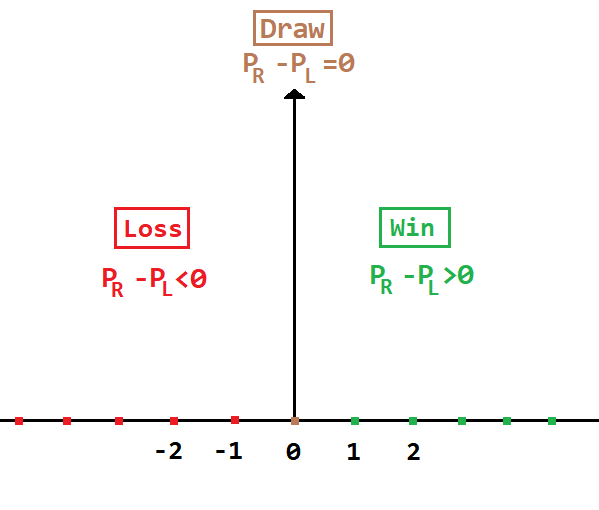
\includegraphics[scale =0.5]{winloss.png}
\caption{An illustration for win or loss conditions for 1-D QW}
\label{fig:win-loss}
\end{figure}

\section{Parrondo's games in quantum walks with a qubit (two state coin)}\label{2state}
\begin{figure}
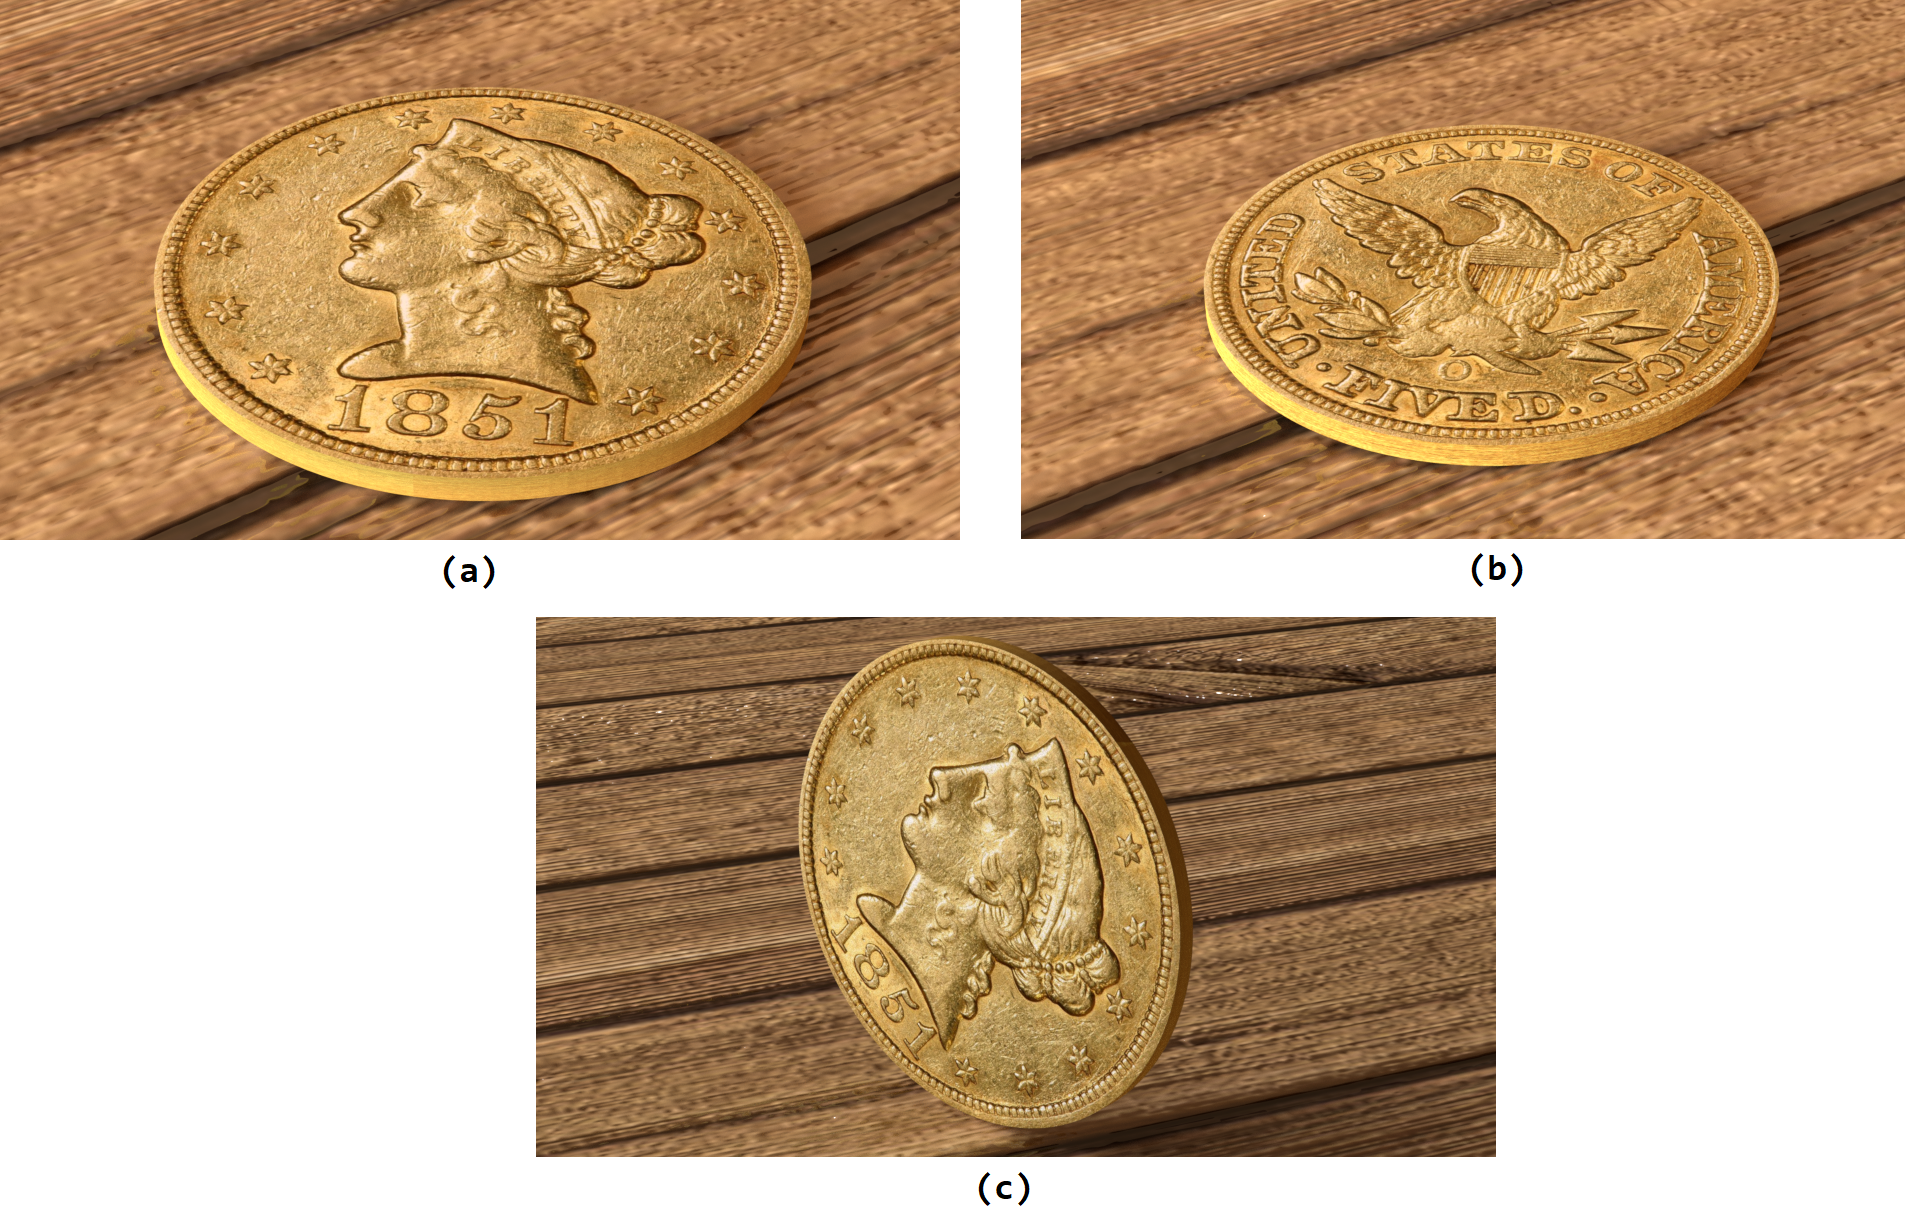
\includegraphics[scale=0.45]{coin.png}
 \caption{ The three states of a coin a) Heads b) Tails and c) Sides}\label{classical_coin}
\end{figure}

In this section, we show why the implementation of Parrond's paradox failed in case of quantum walks with a two-state coin as shown in \cite{minli,flitney}. This part is included as a motivation for our next section to implement a true Parrondo's paradox in quantum walks with a three-state coin.  To understand the reasons behind the failure for seeing a genuine Parrondo's paradox in quantum walks with two state coin is as follows: Two unitary operators $U(\alpha_{A},\beta_{A},\gamma_{A})$ and $U(\alpha_{B},\beta_{B},\gamma_{B})$, representing two games A and B are alternately played according to time,


\begin{equation}
U(\alpha,\beta,\gamma)=\left(\begin{array}{cc}
e^{i\alpha}\cos\beta & -e^{-i\gamma}\sin\beta\\
e^{i\gamma}\sin\beta & e^{-i\alpha}\cos\beta
\end{array}\right).\label{eq:SU(2)}
\end{equation}
The quantum walker is in an initial state $\vert\Psi_{0}\rangle=\frac{1}{\sqrt{2}}\vert 0\rangle_p \otimes(\vert 0\rangle_c +i\vert 1\rangle_c),$ where subscript $p$ refers to the position space and $c$ refers to the single coin space which is initially in  a superposition of $|0\rangle_c$ and $|1\rangle_c$. The dynamics of the walker is governed by a unitary shift operator ($\mathcal{S}$) acting in the position space defined as,
\begin{equation}
\mathcal{S} =   \sum\limits_{n=-\infty}^{\infty}\vert n+1 \rangle_p \langle n \vert_p \otimes \vert 0 \rangle_c \langle 0 \vert_c +   \sum\limits_{n=-\infty}^{\infty}\vert n-1 \rangle_p \langle n \vert_p \otimes \vert 1 \rangle_c \langle 1 \vert_c.
\label{Equ:S}
\end{equation}
The games \emph{A} and \emph{B} can be played in different sequence, i.e., $U(\alpha_{A},\beta_{A},\gamma_{A})$(representing game \emph{A}) is operated on time steps $t=nq$ and $U(\alpha_{B},\beta_{B},\gamma_{B})$(representing game \emph{B}) is operated on time steps $t\neq nq$, where $q$ is the period and $n$ is an integer. This scheme can produce various game sequences like $ABAB\ldots$, $ABBABB\ldots$ etc. The evolution operator can be written as: 
\begin{equation}
U =\left\lbrace 
	\begin{array}{ll}
		\mathcal{S}\cdot (I_p \otimes U(\alpha_{A},\beta_{A},\gamma_{A}))  & \mbox{if } t=nq,n\in Z \\
		\mathcal{S}\cdot (I_p \otimes U(\alpha_{B},\beta_{B},\gamma_{B})) & \mbox{if } t\neq nq,n\in Z
	\end{array}
\right. 
\end{equation}

\begin{figure}[H]
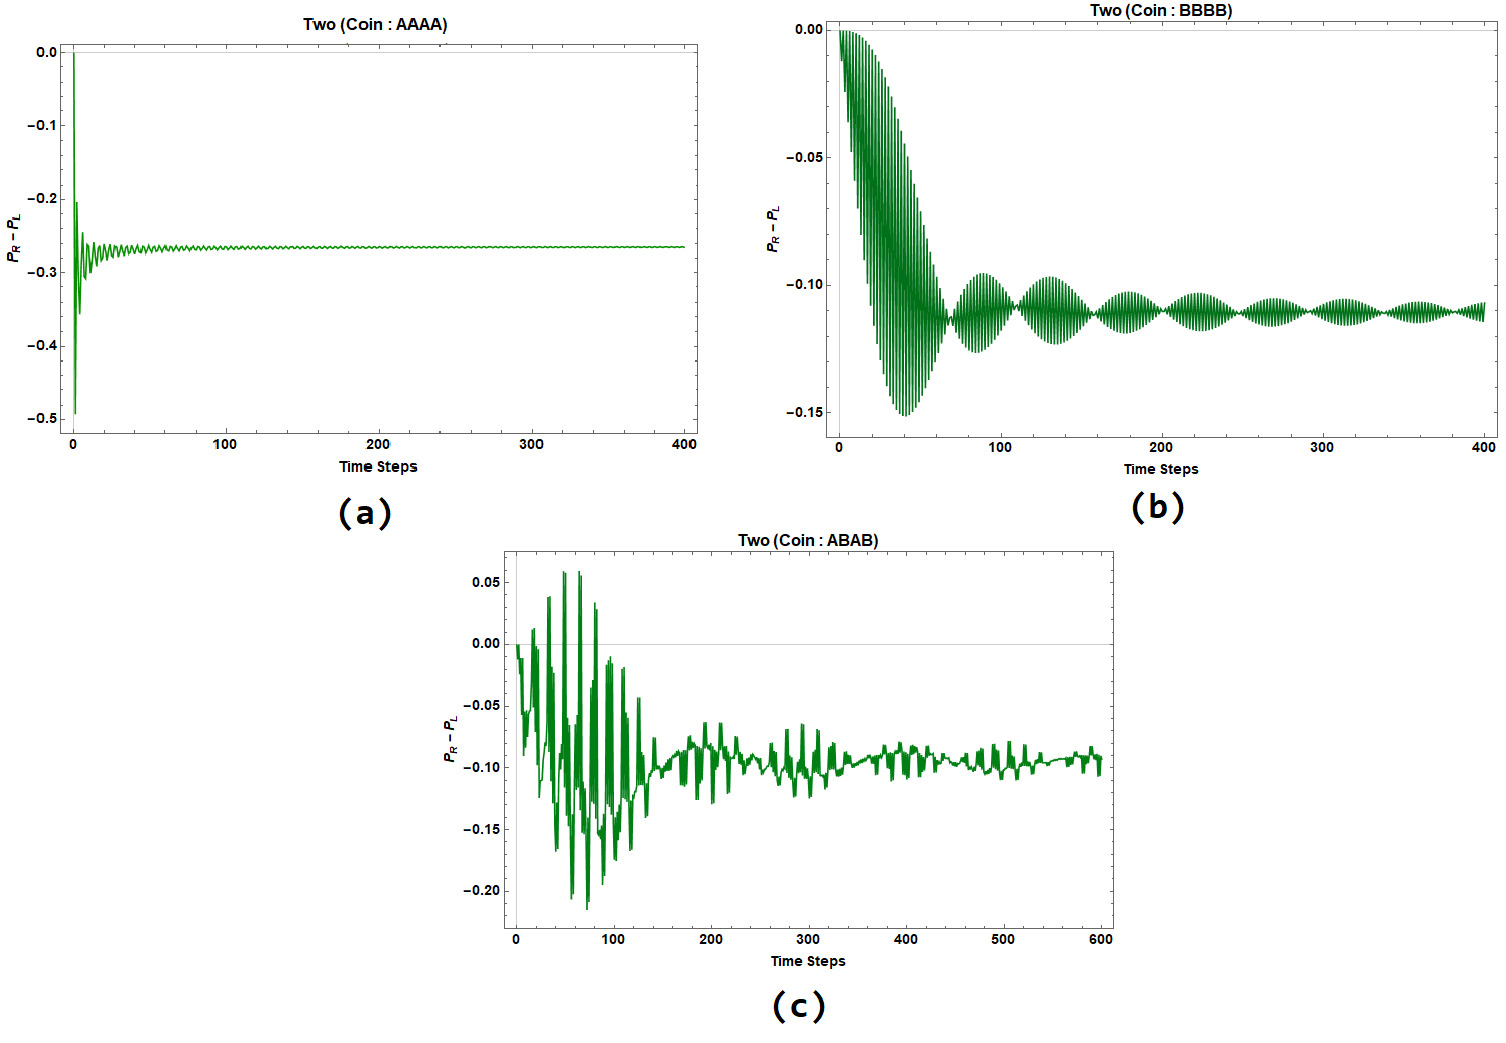
\includegraphics[scale=0.55]{two_state.png}
 \caption{a) $P_R -P_L$ for the sequence $AAAA\ldots$ with initial state $| 0 \rangle_p \otimes \frac{1}{\sqrt{2}}(| 0 \rangle_c - i| 1 \rangle_c)$ with coin operator $A = U(-45, 40, 0)$,  b) $P_R -P_L$ for the sequence $BBBB\ldots$ with initial state $| 0 \rangle_p \otimes \frac{1}{\sqrt{2}}(| 0 \rangle_c - i| 1 \rangle_c)$ with coin operator $B = U(0, 88, -15)$, c) $P_R -P_L$ for the sequence $ABBBABBB\ldots$ with initial state $| 0 \rangle_p \otimes \frac{1}{\sqrt{2}}(| 0 \rangle_c - i| 1 \rangle_c)$ with coin operator $A = U(-45, 40, 0)$ and $B = U(0, 88, -15)$}\label{previous_result}
\end{figure}

and after $N$ steps the final state is given by $\vert\Psi_{N}\rangle=U^{N}\vert\Psi_{0}\rangle$. As illustrated in Fig. \ref{fig:win-loss}, after $N$ steps, if the probability of finding the walker to the right of the origin $P_{R}$, is greater than the probability $P_{L}$ to be found to the left of the origin , i.e., $P_{R}-P_{L}>0$, then the player wins. Similarly, if $P_{R}-P_{L}<0$, the player losses. If $P_{R}-P_{L}=0$, it's a draw. Parrondo's games using 1-D DTQW are formulated by making use of above scheme.Two different biased coin operators $U_{A} (\alpha_{A},\beta_{A},\gamma_{A})$ and $U_{B}(\alpha_{B},\beta_{B},\gamma_{B})$ is used to construct the two losing games \emph{A} and \emph{B}, for $\alpha_A=-45,\beta_{A}=45,\gamma_{A}=0,\alpha_{B}=0,\beta_{B}=88,\gamma_B=-15$, i.e., for $U_{A}=U(-45,45,0)$, $U_{B}=U(0,88,-15)$ we obtain the Fig.\ref{previous_result}. Individually each of the games is losing(See Figure \ref{previous_result}(a),(b))and for the sequences \emph{$ABBBABBB\ldots$} the result is winning at the beginning but in the asymptotic limit the player will lose again as in Fig.\ref{previous_result}(c), one can check for different sequences like \emph{$ABAB\ldots ABBABB\ldots$ etc.} and in all cases in the asymptotic limits we lose. Hence Parrondo's paradox does not exist in case of 1-D DTQW with a two state single coin as established in \cite{minli, flitney}. 


\section{True Parrondo's games in quantum walks with a qutrit(three state coin)}\label{3state}
In this section, we define a one-dimensional discrete time QW with a three-state coin. The position of the walker is defined by a vector in the Hilbert space $\mathcal{H_P}$ spanned by an orthogonal normal basis $\lbrace \vert n \rangle : n \in \mathbb{Z} \rbrace$. At each position, the walker is in a superposition of three coin states. This coin state is a vector in Hilbert space $\mathcal{H_C}$ with basis states represented by the following orthogonal vectors:
\begin{equation}
|1\rangle= \left[  \begin{array}{c}
1 \\ 
0 \\ 
0
\end{array} \right]  , |0\rangle= \left[  \begin{array}{c}
0 \\ 
1 \\ 
0
\end{array} \right]  , |-1\rangle= \left[  \begin{array}{c}
0 \\ 
0 \\ 
1
\end{array} \right]
\end{equation} 
The state of the walker at each time step $t \in \left\lbrace 0,1,2 \ldots \right\rbrace $ $| \psi_t \rangle$ is defined on the Hilbert space $\mathcal{H_P} \otimes \mathcal{H_C}$, the initial state of the walker at time step $t=0$ is 
\begin{equation}\label{initial_1}
|\psi_0 \rangle = | 0 \rangle_p \otimes \frac{1}{\sqrt{3}}(| 0 \rangle_c + | 1 \rangle_c - i| -1 \rangle_c)
\end{equation}
In case of a general walk the position of the walker is shifted by the shift operator $\mathcal{S^{\prime}}$ after the coin operator $\mathcal{C}$ is operated on the superposition as:

\begin{equation}
\vert\psi_{t+1}\rangle= \mathcal{S^{\prime}} \cdot \mathcal{C} \vert\psi_{t}\rangle
\end{equation}
where,
\begin{equation}\label{shift_3}
\mathcal{S^{\prime}} =   \sum\limits_{n=-\infty}^{\infty}\vert n+1 \rangle_p \langle n \vert_p \otimes \vert 0 \rangle_c \langle 0 \vert_c +   \sum\limits_{n=-\infty}^{\infty}\vert n \rangle_p \langle n \vert_p \otimes \vert 1 \rangle_c \langle 1 \vert_c +   \sum\limits_{n=-\infty}^{\infty}\vert n-1 \rangle_p \langle n \vert_p \otimes \vert -1 \rangle_c \langle -1 \vert_c
\end{equation}
The shift operator is defined in such a way that only when the coin is in the state $| 0 \rangle_c$ or $| -1\rangle_c $ the walker moves else when walker is in state $|1\rangle_c$ the walker stays in the same position. The coin operator $\mathcal{C}$ is defined as follows:

\begin{equation}
\mathcal{C}=\mathcal{C}(\alpha, \beta, \gamma, \theta)=\left(  \begin{array}{ccc}
I & J & K \\ 
K & I & J \\ 
J & K & I 
\end{array} \right) + i\left(  \begin{array}{ccc}
R & B & G \\ 
B & G & R \\ 
G & R & B 
\end{array} \right)
\end{equation}


where $\alpha$, $\beta$, $\gamma$ and $\theta$ are four real parameters defining $I, J, K, R, G$ and $B$ where

\begin{equation}
\begin{array}{ll}
3I &= \cos(\gamma) + 2\cos(\theta)\cos(\alpha) \\
3J &= \cos(\gamma) + 2\cos(\theta)\cos(\alpha + 2\pi/3)\\
3K &= \cos(\gamma) + 2\cos(\theta)\cos(\alpha + \pi/3) \\
3R &= \sin(\gamma) + 2\sin(\theta)\cos(\beta) \\
3G &= \sin(\gamma) + 2\sin(\theta)\cos(\beta + 2\pi/3) \\
3B &= \sin(\gamma) + 2\sin(\theta)\cos(\beta + 4\pi/3) 
\end{array}
\end{equation}
This kind of unitary operators are used in particle physics in the density matrix formalism for elementary particles\cite{particle_phy}.\\

Similar to that of two state coin QW scheme discussed in section \ref{2state}, we define an evolution operator as follows:
\begin{equation}
U^{\prime} =\left\lbrace 
	\begin{array}{ll}
		\mathcal{S^{\prime}}\cdot (I_p \otimes \mathcal{C}(\alpha_A, \beta_A, \gamma_A, \theta_A))  & \mbox{if } t=nq,n\in Z \\
		\mathcal{S^{\prime}}\cdot (I_p \otimes \mathcal{C}(\alpha_B, \beta_B, \gamma_B, \theta_B))  & \mbox{if } t\neq nq,n\in Z.
	\end{array}
\right.  
\end{equation}
The above definitions of coin operator, shift operator and evolution operator incorporates the stochastic behavior of the quantum walks with a three state coin. The evolution of the walker after $N$ steps is $|\psi_N\rangle = U^{\prime N}|\psi_0\rangle$. Similar to that of the two state coin quantum walks, winning and losing is defined as follows: if the probability of finding the walker to the right of the origin $P_{R}$, is greater than the probability $P_{L}$ to be found to the left of the origin , i.e., $P_{R}-P_{L}>0$, then the player wins. Similarly, if $P_{R}-P_{L}<0$, the player losses. If $P_{R}-P_{L}=0$, it's a draw. The two coin operators corresponding to the two games $A$ and $B$ are defined as follows:

\begin{equation}\label{coin_operator}
\begin{array}{ll}
A &= \mathcal{C}(\alpha_A, \beta_A, \gamma_A, \theta_A) = \mathcal{C}(\pi, \frac{\pi}{2}, \pi, \pi) \\
B &= \mathcal{C}(\alpha_B, \beta_B, \gamma_B, \theta_B) = \mathcal{C}(\frac{\pi}{2}, \frac{\pi}{2}, \frac{3\pi}{2}, \frac{\pi}{2})
\end{array}
\end{equation}

Here $A$ is operated on time steps
$t=nq$ and $B$ is played on time steps $t\neq nq$, where $q$ is the period and $n$ is an integer same as discussed in section \ref{2state}. For the choice of $\alpha_A=\pi,\beta_{A}=\pi/2,\gamma_{A}=\pi,\theta_{A}=\pi, \alpha_{B}=\pi/2,\beta_{B}=\pi/2,\gamma_B=3\pi/2, \theta=\pi/2$ as shown in Eq.\ref{coin_operator} we obtain the Fig.\ref{result}. When game AAAA... and BBBB... are played it results in losing(See Figs.\ref{result}(a),(b)), whereas when they were played in the sequence $ABAB\ldots$ we obtain Fig.\ref{result}(c) where we get a winning outcome. Thus unlike in two state coin, in case of a three state coin in asymptotic limits we obtain a true Parrondo's paradox.
\begin{figure}[H]
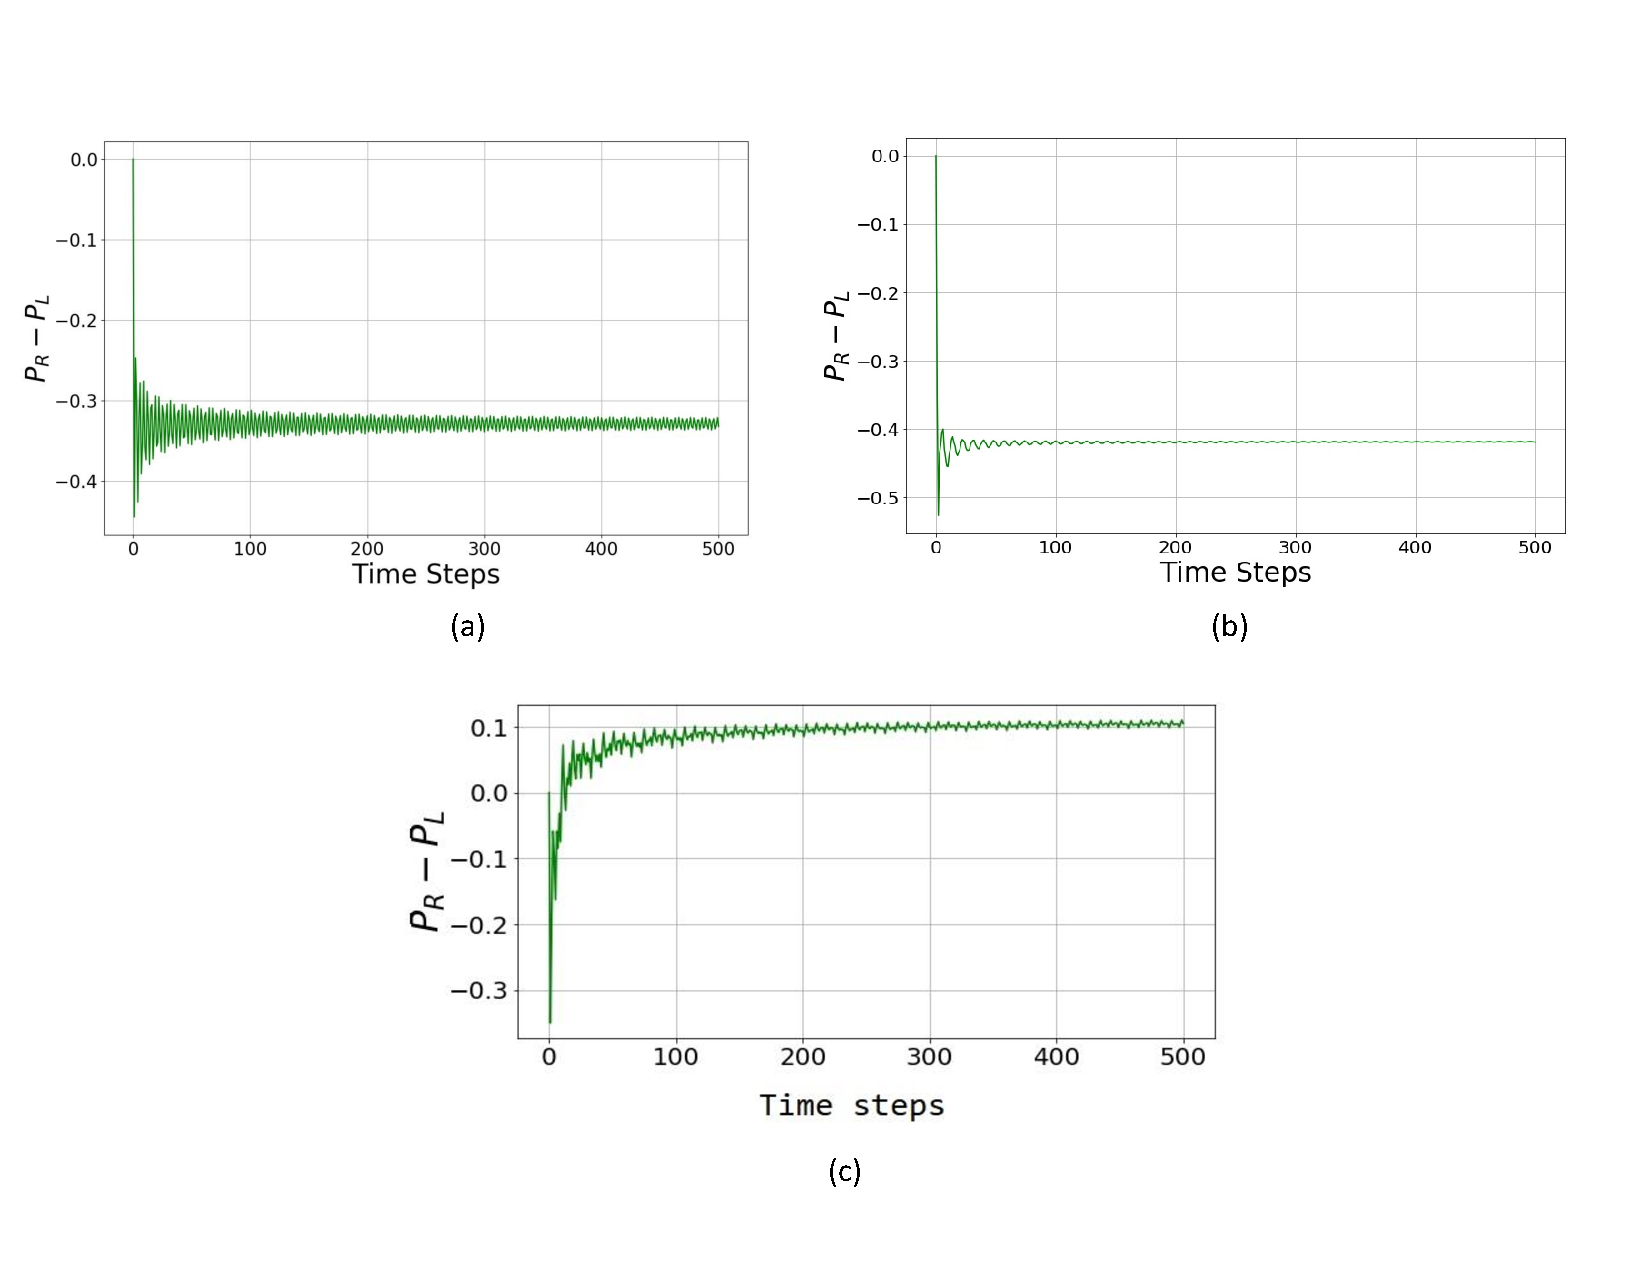
\includegraphics[scale=0.6]{3state_plot.pdf}
 \caption{a) $P_R -P_L$ for the sequence $AAAA\ldots$ with initial state $| 0 \rangle_p \otimes \frac{1}{\sqrt{3}}(| 0 \rangle_c + | 1 \rangle_c - i| -1 \rangle_c)$ with coin operator $A = \mathcal{C}(\pi, \pi/2, \pi, \pi)$  b) $P_R -P_L$ for the sequence $BBBB\ldots$ with initial state $| 0 \rangle_p \otimes \frac{1}{\sqrt{3}}(| 0 \rangle_c + | 1 \rangle_c - i| -1 \rangle_c)$ with coin operator $B = \mathcal{C}(\pi/2, \pi/2, 3\pi/2, \pi/2)$ c) $P_R -P_L$ for the sequence $ABAB\ldots$ with initial state $| 0 \rangle_p \otimes \frac{1}{\sqrt{3}}(| 0 \rangle_c + | 1 \rangle_c - i| -1 \rangle_c)$ with coin operator $A = \mathcal{C}(\pi, \pi/2, \pi, \pi)$ and $B = \mathcal{C}(\pi/2, \pi/2, 3\pi/2, \pi/2)$ for 500 steps}\label{result}
\end{figure}
\section{Discussion}\label{discussion}

When a two-state coin(qubit) was considered the Parrondo's games did not give rise to the paradox in asymptotic limits(Fig.\ref{previous_result}) whereas when a three-state coin is used for quantum walks we obtain a true Parrondo's paradox. In order to obtain a true Parrondo's paradox, a three-state coin is needed. In Refs.\cite{minli,flitney} it was shown that in asymptotic limits for a two-state coin the paradox does not exist. To identify the reasons for the success of three state coin as compared to a two-state coin we study the influence of the initial state in the Parrondo's games. Consider an initial state given as:
\begin{equation}\label{new_initial}
|\psi_0 \rangle = | 0 \rangle_p \otimes \frac{1}{\sqrt{3}}(| 1 \rangle_c +| 0 \rangle_c - | -1 \rangle_c)
\end{equation} 
This is different from the initial state Eq.\ref{initial_1}, 
for the same shift $\mathcal{S^{\prime}}$ (Eq.\ref{shift_3}) defined as in Section \ref{3state} we now obtain the Figure.\ref{initial_state} for initial state Eq.\ref{new_initial}. It is clear that the new initial state does not give us a paradox, when the games are played in sequence $ABAB\ldots$(See Figure \ref{initial_state}(c)). This implies that the initial state plays a crucial role in the Parrondo's games, with different initial states one may or may not obtain a true Parrondo's paradox.\\

\begin{figure}[h]
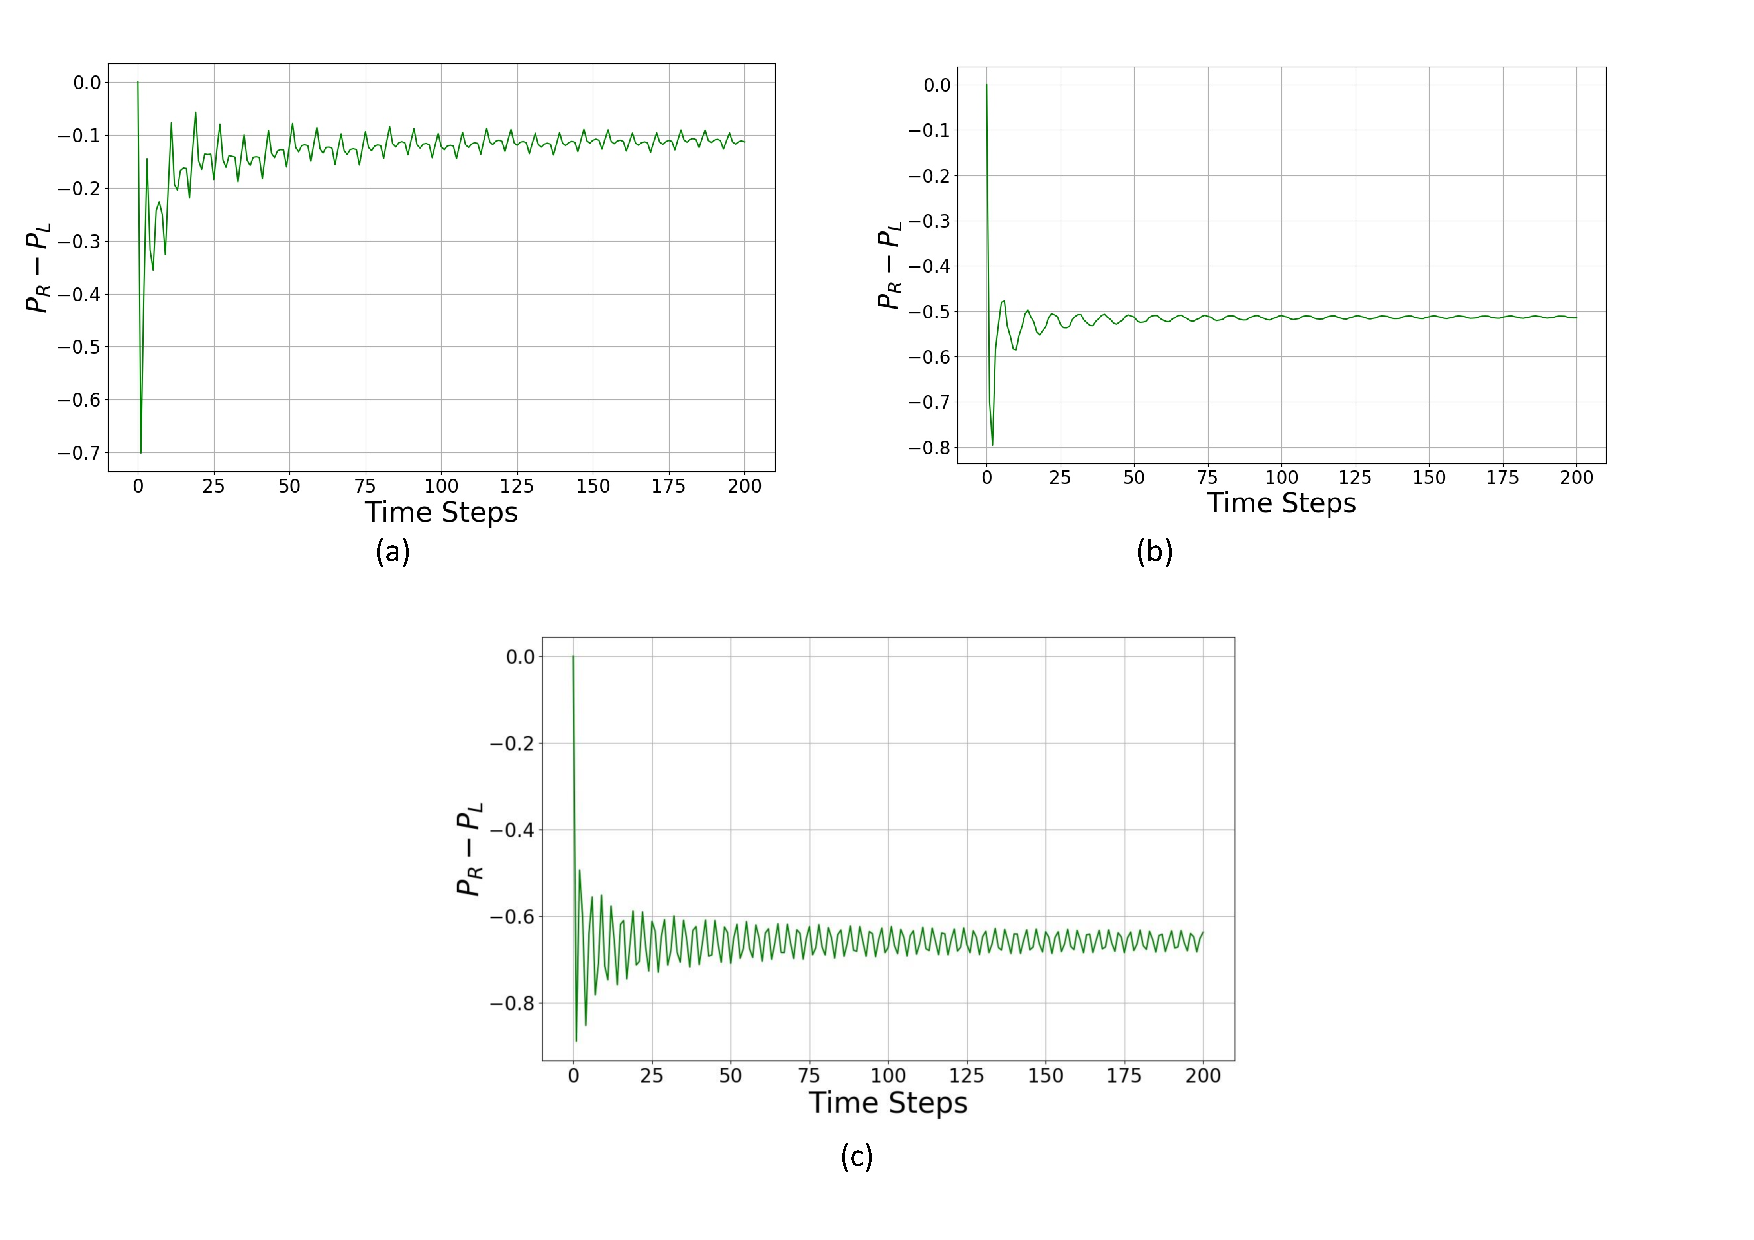
\includegraphics[scale=0.6]{3state_diff_initial.pdf}

 \caption{a) $P_R -P_L$ for the sequence $AAAA\ldots$ with initial state $| 0 \rangle_p \otimes \frac{1}{\sqrt{3}}(| 1 \rangle_c + | 0 \rangle_c - | -1 \rangle_c)$ with coin operator $A = \mathcal{C}(\pi, \pi/2, \pi, \pi)$  b) $P_R -P_L$ for the sequence $BBBB\ldots$ with initial state $| 0 \rangle_p \otimes \frac{1}{\sqrt{3}}(| 1 \rangle_c + | 0 \rangle_c - | -1 \rangle_c)$ with coin operator $B = \mathcal{C}(\pi/2, \pi/2, 3\pi/2, \pi/2)$ c) $P_R -P_L$ for the sequence $ABAB\ldots$ with initial state $| 0 \rangle_p \otimes \frac{1}{\sqrt{3}}(| 1 \rangle_c + | 0 \rangle_c - | -1 \rangle_c)$ with coin operator $A = \mathcal{C}(\pi, \pi/2, \pi, \pi)$ and $B = \mathcal{C}(\pi/2, \pi/2, 3\pi/2, \pi/2)$ for 200 steps}\label{initial_state}
\end{figure}
Now we consider the influence of the shift operator. Using a different shift operator for the same initial states as in Section \ref{3state}. Here we define a new shift $\mathcal{S^{\prime}_\texttt{1}}$ -
\begin{equation}\label{new_shift}
\mathcal{S^{\prime}_\texttt{1}} =   \sum\limits_{n=-\infty}^{\infty}\vert n+1 \rangle_p \langle n \vert_p \otimes \vert  1\rangle_c \langle 1 \vert_c +   \sum\limits_{n=-\infty}^{\infty}\vert n \rangle_p \langle n \vert_p \otimes \vert 0 \rangle_c \langle 0 \vert_c +   \sum\limits_{n=-\infty}^{\infty}\vert n-1 \rangle_p \langle n \vert_p \otimes \vert -1 \rangle_c \langle -1 \vert_c
\end{equation}

\begin{figure}[H]
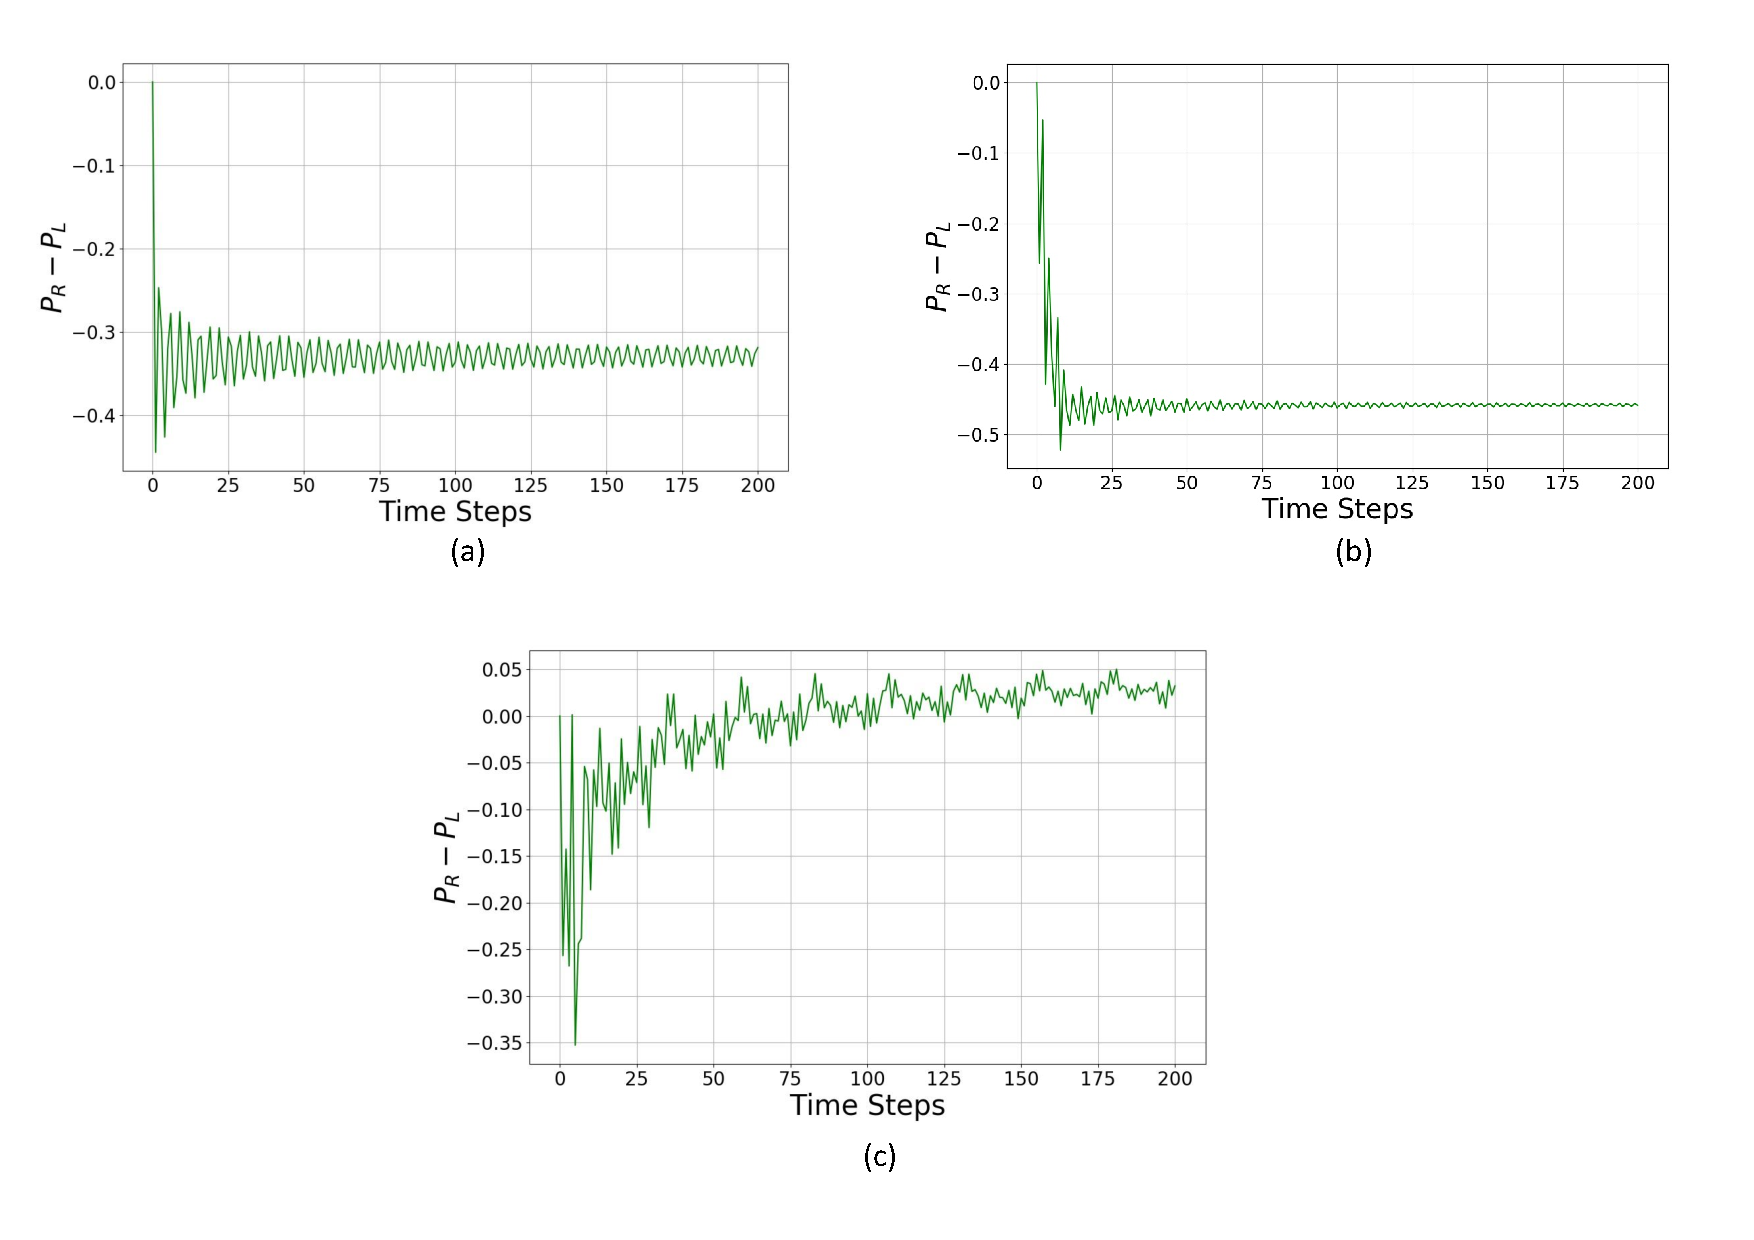
\includegraphics[scale=0.65]{diff_shift_1.pdf}
 \caption{a) $P_R -P_L$ for the sequence $AAAA\ldots$ with initial state $| 0 \rangle_p \otimes \frac{1}{\sqrt{3}}(| 1 \rangle_c + | 0 \rangle_c - i | -1 \rangle_c)$ with coin operator $A = \mathcal{C}(\pi, \pi/2, \pi, \pi)$  b) $P_R -P_L$ for the sequence $BBBB\ldots$ with initial state $| 0 \rangle_p \otimes \frac{1}{\sqrt{3}}(| 1 \rangle_c + | 0 \rangle_c - i| -1 \rangle_c)$ with coin operator $B = \mathcal{C}(\pi/2, \pi/2, 3\pi/2, \pi/2)$ c) $P_R -P_L$ for the sequence $ABAB\ldots$ with initial state $| 0 \rangle_p \otimes \frac{1}{\sqrt{3}}(| 1 \rangle_c + | 0 \rangle_c - i| -1 \rangle_c)$ with coin operator $A = \mathcal{C}(\pi, \pi/2, \pi, \pi)$ and $B = \mathcal{C}(\pi/2, \pi/2, 3\pi/2, \pi/2)$ for the shift operator $\mathcal{S^{\prime}_\texttt{1}}$ defined in Eq. \ref{new_shift}}\label{shift1}
\end{figure}
The shift operator defined as in Eq. \ref{new_shift} with one wait state also gives us a Parrondo's paradox after around 200 steps(almost asymptotic limit) as in Fig.\ref{shift1}. One can see that the change in shift operator has changed the behavior of the Parrondo's games, here the yield of the player is changing. Now if we consider the shift operator $\mathcal{S^{\prime}_\texttt{2}}$ 
\begin{equation}\label{new_shift2}
\mathcal{S^{\prime}_\texttt{2}} =   \sum\limits_{n=-\infty}^{\infty}\vert n+1 \rangle_p \langle n \vert_p \otimes \vert  1\rangle_c \langle 1 \vert_c +   \sum\limits_{n=-\infty}^{\infty}\vert n-1 \rangle_p \langle n \vert_p \otimes \vert 0 \rangle_c \langle 0 \vert_c +   \sum\limits_{n=-\infty}^{\infty}\vert n \rangle_p \langle n \vert_p \otimes \vert -1 \rangle_c \langle -1 \vert_c
\end{equation}

\begin{figure}
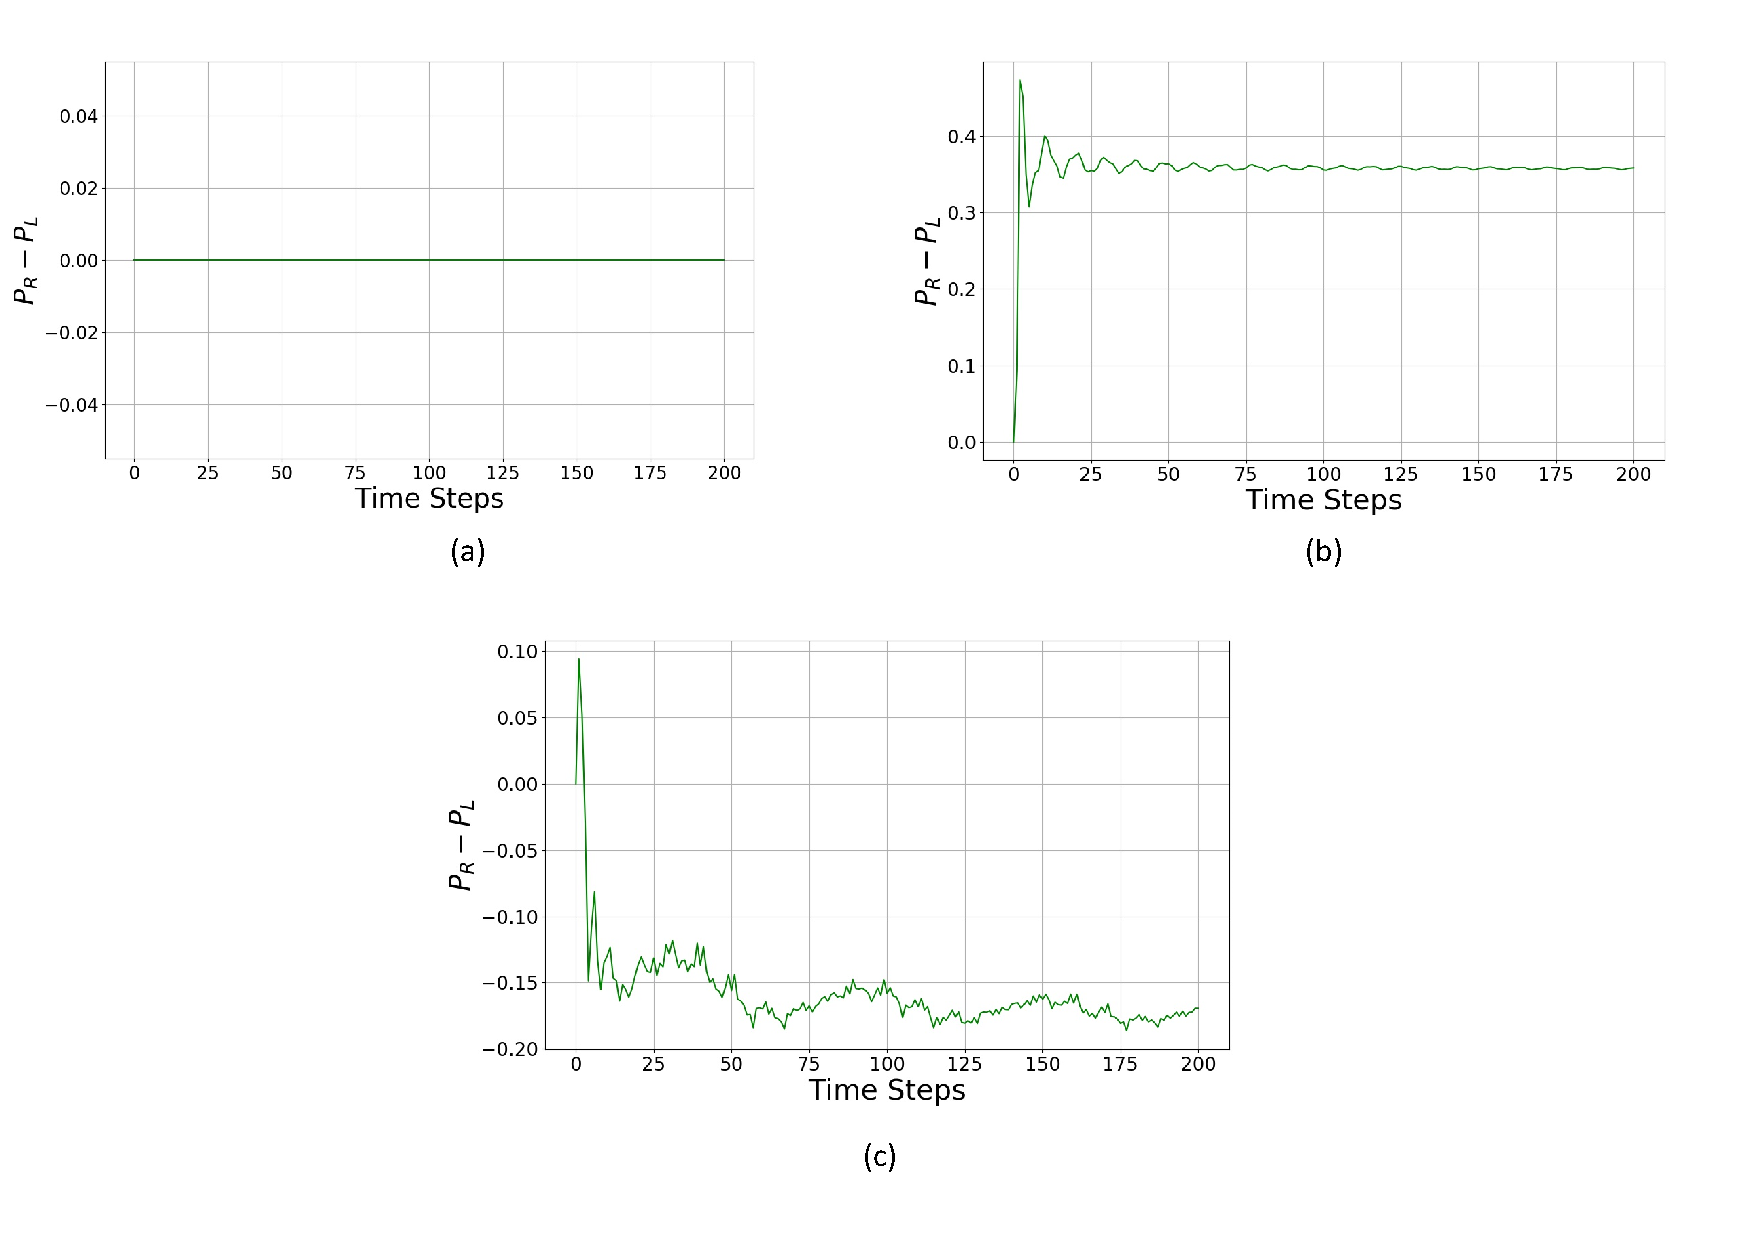
\includegraphics[scale=0.65]{diff_shift.pdf}
 \caption{a) $P_R -P_L$ for the sequence $AAAA\ldots$ with initial state $| 0 \rangle_p \otimes \frac{1}{\sqrt{3}}(| 1 \rangle_c + | 0 \rangle_c - i | -1 \rangle_c)$ with coin operator $A = \mathcal{C}(\pi, \pi/2, \pi, \pi)$  b) $P_R -P_L$ for the sequence $BBBB\ldots$ with initial state $| 0 \rangle_p \otimes \frac{1}{\sqrt{3}}(| 1 \rangle_c + | 0 \rangle_c - i| -1 \rangle_c)$ with coin operator $B = \mathcal{C}(\pi/2, \pi/2, 3\pi/2, \pi/2)$ c) $P_R -P_L$ for the sequence $ABAB\ldots$ with initial state $| 0 \rangle_p \otimes \frac{1}{\sqrt{3}}(| 1 \rangle_c + | 0 \rangle_c - i| -1 \rangle_c)$ with coin operator $A = \mathcal{C}(\pi, \pi/2, \pi, \pi)$ and $B = \mathcal{C}(\pi/2, \pi/2, 3\pi/2, \pi/2)$ for the shift operator $\mathcal{S^{\prime}_\texttt{1}}$ defined in Eq. \ref{new_shift2}}\label{shift2}
\end{figure}

where the state $\vert -1 \rangle$ is the wait state, we obtain the Fig.\ref{shift2}. Here the game sequence $AAAA\ldots$ gives us a draw and the sequence $BBBB\ldots$ provides a winning outcome whereas the $ABAB\ldots$ sequence gives us a losing outcome, which is also a paradox with a role reversal with the definitions of win and loss from Fig.\ref{fig:win-loss} is reversed. Thus we can conclude that the change of shift operator does not affect the paradox but only the yield of the player. It is the initial three state which is the reason for obtaining a genuine Parrondo's paradox.   


\section{Conclusion}\label{conclusion}
Earlier attempts using a single two-state coin failed in asymptotic limit \cite{minli,flitney}. Here with the aid of a three-state coin(qutrit) we successfully implemented a true Parrondo's paradox(See Fig. \ref{3state}). Quantum Parrondo's games play an important role in quantum ratchets, providing a mechanism for a particle to transport against an applied bias, quantum analogue for Brownian ratchets. Different kinds of quantum walks and its applications can help the community in better understanding and for developing new quantum algorithms.



\begin{thebibliography}{99}
\bibitem{two_particle}
A.~Schreiber, A.~G´abris, P.~P.~Rohde, K.~Laiho, M.~Stefanak, V.~Potocek, C.~Hamilton, I.~Jex, and C.~Silberhorn, A 2D quantum
walk simulation of two-particle dynamics, Science 336, 55
(2012).
\bibitem{Marquez-Martin2016}
I.~M\'arquez-Martín, G.~Di Molfetta, and A.~P\'erez, Fermion confinement via quantum walks in $(2+1)$-dimensional and $(3+1)$-dimensional space-time, Phys. Rev. A 95, 042112 (2017)

\bibitem{algo}
A.~Ambainis, Quantum walks and their algorithmic applications, Int. Journal of Quantum Information 1 (4) (2003) 507

\bibitem{qcomp1}
A.~M. Childs, R. Cleve, E. Deotto, E. Farhi, S. Gutmann, D.A. Spielman, in: Proceedings of the 35th ACM Symposium on Theory of Computing, ACM Press, New York, 2003, p. 59.

\bibitem{qcomp2}
N. Shenvi, J. Kempe, K.~B. Whaley, Quantum random-walk search algorithm. \pra 67 (2003) 052307.

\bibitem{universal}
Andrew M.~Childs, Universal Computation by Quantum Walk, Phys. Rev. Lett. 102, 180501 

\bibitem{classical}
R.~Portugal, Quantum Walks and Search Algorithms, Springer, Berlin 10.1007/978-1-4614-6336-8 (2013) 


\bibitem{Andraca}
S.~E.~Venegas-Andraca, Quantum walks: a comprehensive review , Quantum Information Processing October 2012, Volume 11, Issue 5, pp 1015-1106.

\bibitem{qutrit1}
T.~Machida, C.~M.~ Chandrashekar. Localization and limit laws of a three-state alternate quantum walk on a two-dimensional lattice, \pra 92, 062307 (2015)

\bibitem{qutrit2}
M. \v Stefa\v n\'ak,I. Bezd\v ekov\'a, I. Jex, Limit distributions of three-state quantum walks: the role of coin eigenstates, \pra 90, 012342 (2014)

\bibitem{q_game}
David A. Meyer, Quantum Strategies, \prl 82 (1999) 1052–1055

\bibitem{parrondo}
J.~M.~R.~Parrondo and L.~Dinis, Brownian motion and gambling: from ratchets to paradoxical games, Contemporary Physics, Vol 45, pp. 147-157, 2004.

\bibitem{minli}
M.~Li, Y.~S.~Zhang, G.-C.~Guo, Quantum Parrondo's games constructed by quantum random walk, arXiv:quant-ph/1303.6831 (2013).

\bibitem{flitney} 
A.~P.~Flitney, Quantum Parrondo's games using quantum walks, arXiv:1209.2252 (2012).

\bibitem{previous}
J. Rajendran, C. Benjamin, How to implement a genuine Parrondo's paradox with quantum walks?, arXiv:1702.05927 (2017)

\bibitem{particle_phy}
C. Brannen, Density Operator Theory and Elementary Particles, available at:\url{http://www.brannenworks.com/densitytime.pdf}

\end{thebibliography}
\end{document}

